% ============================================================
%  Statistika e Aplikuar (MFM2S11) — Template Beamer (Singapore)
%  FIMIF · UPT  |  Assoc. Prof. Endri Raço, PhD
%  Kompilim: pdflatex (2 herë, për navigimin Singapore)
%  Logo: logo_upt.png dhe logo_fimif.png (në logos/ ose në të njëjtën dosje).
%        Nëse mungojnë, shfaqet një vend-mbajtës i thjeshtë.
% ============================================================
\documentclass[aspectratio=169,10pt,xcolor={dvipsnames,table}]{beamer}

% ---------- Tema ----------
\usetheme{Singapore}
\setbeamertemplate{navigation symbols}{}
\setbeamertemplate{footline}[frame number]

% ---------- Ngjyrat (blu UPT + ngjyra theksi) ----------
\definecolor{uptblue}{HTML}{1E325A}
\definecolor{uptmid}{HTML}{2C5AA0}
\definecolor{uptlight}{HTML}{E8EEF7}
\definecolor{accent}{HTML}{D97706}
\definecolor{okgreen}{HTML}{15803D}
\definecolor{warnred}{HTML}{B91C1C}
\definecolor{codebg}{HTML}{F6F8FA}

\setbeamercolor{palette primary}{bg=uptblue,fg=white}
\setbeamercolor{palette secondary}{bg=uptmid,fg=white}
\setbeamercolor{palette tertiary}{bg=uptblue,fg=white}
\setbeamercolor{section in head/foot}{bg=uptlight,fg=uptblue}
\setbeamercolor{frametitle}{fg=uptblue,bg=white}
\setbeamercolor{title}{fg=uptblue}
\setbeamercolor{structure}{fg=uptmid}
\setbeamercolor{item}{fg=accent}
\setbeamercolor{block title}{bg=uptmid,fg=white}
\setbeamercolor{block body}{bg=uptlight}
\setbeamerfont{frametitle}{series=\bfseries,size=\large}

% ---------- Paketat ----------
\usepackage[utf8]{inputenc}
\usepackage[T1]{fontenc}
\usepackage{lmodern}
\usepackage{amsmath,amssymb,bm}
\usepackage{booktabs}
\usepackage{graphicx}
\usepackage{tikz}
\usetikzlibrary{positioning,arrows.meta,shapes.geometric,calc,trees}
\usepackage{pgfplots}
\pgfplotsset{compat=1.18}
\usepackage[most]{tcolorbox}
\usepackage{listings}
\usepackage{hyperref}
\hypersetup{colorlinks=true,linkcolor=uptmid,urlcolor=uptmid}

% ---------- Kutitë pedagogjike ----------
\newtcolorbox{Definicion}[1][]{colback=uptlight,colframe=uptblue,fonttitle=\bfseries,title={Definicion #1},boxrule=0.6pt,arc=2pt,left=4pt,right=4pt,top=2pt,bottom=2pt}
\newtcolorbox{Teoreme}[1][]{colback=white,colframe=uptmid,fonttitle=\bfseries,title={Teoremë #1},boxrule=0.6pt,arc=2pt}
\newtcolorbox{Shembull}[1][]{colback=green!4,colframe=okgreen,fonttitle=\bfseries,title={Shembull #1},boxrule=0.6pt,arc=2pt}
\newtcolorbox{Ushtrim}[1][]{colback=orange!5,colframe=accent,fonttitle=\bfseries,title={Radha jote! #1},boxrule=0.6pt,arc=2pt}
\newtcolorbox{Gabim}[1][]{colback=red!4,colframe=warnred,fonttitle=\bfseries,title={Gabim i zakonshëm #1},boxrule=0.6pt,arc=2pt}
\newtcolorbox{Keshille}[1][]{colback=yellow!6,colframe=yellow!50!black,fonttitle=\bfseries,title={Këshillë #1},boxrule=0.6pt,arc=2pt}
\newtcolorbox{Parashiko}[1][]{colback=purple!4,colframe=purple!70!black,fonttitle=\bfseries,title={Parashiko para se ta ekzekutosh #1},boxrule=0.6pt,arc=2pt}

% ---------- Stili i kodit R ----------
\lstdefinestyle{Rstyle}{
  language=R,
  backgroundcolor=\color{codebg},
  basicstyle=\ttfamily\footnotesize,
  keywordstyle=\color{uptmid}\bfseries,
  commentstyle=\color{gray}\itshape,
  stringstyle=\color{okgreen},
  showstringspaces=false,
  frame=single, rulecolor=\color{uptlight},
  breaklines=true, columns=fullflexible,
  numbers=left, numberstyle=\tiny\color{gray}, numbersep=6pt,
  xleftmargin=12pt, framexleftmargin=12pt,
  literate={ë}{{\"e}}1 {Ë}{{\"E}}1 {ç}{{\c c}}1 {Ç}{{\c C}}1 {<-}{{$\leftarrow$}}1
}
\lstset{style=Rstyle}
\lstdefinestyle{Rout}{columns=fixed,keepspaces=true,basicstyle=\ttfamily\footnotesize\color{uptblue},backgroundcolor=\color{white},frame=leftline,rulecolor=\color{accent},numbers=none,xleftmargin=8pt}

% ---------- Komanda ndihmëse ----------
\newcommand{\Rkey}[1]{\texttt{\textcolor{uptmid}{#1}}}
\newcommand{\termi}[2]{\textbf{#1} (\emph{#2})}
\newcommand{\shkoTe}[2]{\hyperlink{#1}{\beamergotobutton{#2}}}
\newcommand{\kthehu}[1]{\hyperlink{#1}{\beamerreturnbutton{Kthehu}}}
\newcommand{\Zgjerim}{\colorbox{accent}{\textcolor{white}{\tiny\bfseries ZGJERIM}}\ }  % etiketë për materialin që mund të shkurtohet
\newcommand{\Plotesues}{\colorbox{uptmid}{\textcolor{white}{\tiny\bfseries MATERIAL PLOTËSUES}}\ }  % tema jashtë repo-s ISLR

% ---------- Logo (vend-mbajtës nëse mungon skedari) ----------
\newcommand{\logoUPT}{%
  \IfFileExists{logos/logo_upt.png}{
\includegraphics[height=0.9cm]{logos/logo_upt.png}}{%
  \tikz{\node[draw=uptblue,thick,rounded corners=2pt,minimum width=1.6cm,minimum height=0.8cm,font=\scriptsize\bfseries,text=uptblue]{UPT};}}}
\newcommand{\logoFIMIF}{%
  \IfFileExists{logos/logo_fimif.png}{
\includegraphics[height=0.9cm]{logos/logo_fimif.png}}{%
  \tikz{\node[draw=uptmid,thick,rounded corners=2pt,minimum width=1.6cm,minimum height=0.8cm,font=\scriptsize\bfseries,text=uptmid]{FIMIF};}}}

% ---------- Informacioni i leksionit (ndrysho çdo javë) ----------
\newcommand{\javaNr}{1}
\newcommand{\temaJaves}{Hyrje në R dhe RStudio; vizualizimi bazë}
\title[SA · Java \javaNr]{Statistika e Aplikuar}
\subtitle{Java \javaNr: \temaJaves}
\author{Assoc. Prof. Endri Raço, PhD}
\institute{Fakulteti i Inxhinierisë Matematike dhe Inxhinierisë Fizike\\Universiteti Politeknik i Tiranës}
\date{Workshop 7-orësh}
\titlegraphic{\logoUPT\hspace{0.6cm}\logoFIMIF}

\begin{document}

% ===================== FAQJA E TITULLIT =====================
\begin{frame}[plain]
  \titlepage
\end{frame}

\begin{frame}{Plani i ditës (7 orë)}
  \tableofcontents
\end{frame}

% ===================== ORA 1 =====================
\section{Motivimi}
\subsection{Problemi real}

\begin{frame}{Pse na duhet regresi?}
  \begin{itemize}
    \item<1-> Një firmë do të dijë si ndikon \textbf{reklama} te shitjet.
    \item<2-> Të dhënat: buxheti TV, radio, gazeta dhe shitjet.
    \item<3-> Pyetja: sa rriten shitjet për çdo 1\,000 \$ më shumë në TV?
  \end{itemize}
  \onslide<4->{\begin{Keshille}Mbaje mend këtë pyetje: i përgjigjemi në Orën 6 me të dhënat Advertising.\end{Keshille}}
\end{frame}

\subsection{Objektivat}
\begin{frame}{Objektivat e mësimit (K2, S2, S4)}
  Në fund të ditës do të jesh në gjendje:
  \begin{enumerate}
    \item të shpjegosh \termi{katrorët më të vegjël}{least squares};
    \item të vlerësosh modelin në R me \Rkey{lm()};
    \item të interpretosh $\hat\beta_1$ dhe \termi{koeficientin e përcaktimit}{coefficient of determination} $R^2$.
  \end{enumerate}
\end{frame}

% ===================== ORA 2 =====================
\section{Teoria}
\subsection{Përkufizime}

\begin{frame}{Modeli i thjeshtë linear}
  \begin{Definicion}[(Modeli)]
    \[ Y_i=\beta_0+\beta_1 x_i+\varepsilon_i,\qquad \varepsilon_i\sim N(0,\sigma^2) \]
  \end{Definicion}
  \pause
  \begin{itemize}
    \item $\beta_0$ = prerja; $\beta_1$ = pjerrësia.
    \pause
    \item $\varepsilon_i$ = gabimi i rastit për vrojtimin $i$.
  \end{itemize}
\end{frame}

\begin{frame}{Vlerësuesit OLS: hap pas hapi}
  \begin{align*}
    \hat\beta_1 &= \frac{\sum_{i}(x_i-\bar x)(y_i-\bar y)}{\sum_{i}(x_i-\bar x)^2} \\
    \onslide<2->{\hat\beta_0 &= \bar y-\hat\beta_1\bar x}
  \end{align*}
  \onslide<3->{
  \begin{Teoreme}[(Gauss--Markov)]
    Nën supozimet klasike, OLS është vlerësuesi linear i pazhvendosur me variancë më të vogël.
  \end{Teoreme}}
  \onslide<4->{
  \begin{Gabim}$R^2$ i lartë nuk do të thotë shkakësi.\end{Gabim}}
\end{frame}

% ===================== ORA 3 =====================
\section{Laborator R}
\subsection{Nga zero}

\begin{frame}[fragile]{Kodi R: vlerësimi i modelit}
\begin{lstlisting}
set.seed(2026)                    # reproducibility
ads <- read.csv("Advertising.csv")  # ISLR website, not in ISLR2
fit <- lm(sales ~ TV, data = ads)
coef(summary(fit))
\end{lstlisting}
\end{frame}

\begin{frame}[fragile]{Çfarë na tregon rezultati?}
\begin{lstlisting}[style=Rout]
[Output: ekzekuto në RStudio]
\end{lstlisting}
  \footnotesize\textcolor{gray}{(Në leksion shfaqet vetëm output-i i ekzekutuar realisht nga knitr.)}
\end{frame}

\begin{frame}[label=pyetja1]{Parashiko!}
  \begin{Parashiko}
    Nëse $\hat\beta_1=0.05$, sa ndryshojnë shitjet kur TV rritet me 100?\\[2pt]
    \textbf{A)} 0.05 \quad \textbf{B)} 5 \quad \textbf{C)} 50
  \end{Parashiko}
  \shkoTe{zgjidhja1}{Shiko zgjidhjen}
\end{frame}

% ===================== ORA 4 =====================
\section{Ilustrime}
\subsection{Grafika}

\begin{frame}{\Zgjerim Drejtëza e regresit (pgfplots)}
  \centering
  \begin{tikzpicture}
    \begin{axis}[width=0.7\textwidth,height=0.55\textheight,
      xlabel={$x$},ylabel={$y$},grid=major,grid style={gray!20}]
      \addplot[only marks,mark=*,uptmid] coordinates {(1,2) (2,3) (3,5) (4,4) (5,6)};
      \addplot[accent,very thick,domain=0.5:5.5]{1.3+0.9*x};
    \end{axis}
  \end{tikzpicture}
  \[ \bar x=3,\ \bar y=4,\ \hat\beta_1=\tfrac{9}{10}=0.9,\ \hat\beta_0=4-0.9\cdot 3=1.3 \]
\end{frame}

\begin{frame}{\Plotesues Rrjedha e analizës (TikZ)}
  \centering
  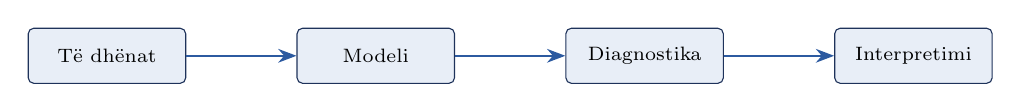
\begin{tikzpicture}[>=Stealth,node distance=1.4cm,
      nd/.style={rectangle,rounded corners=2pt,draw=uptblue,fill=uptlight,minimum width=2cm,minimum height=7mm,font=\scriptsize}]
    \node[nd] (a) {Të dhënat};
    \node[nd,right=of a] (b) {Modeli};
    \node[nd,right=of b] (c) {Diagnostika};
    \node[nd,right=of c] (d) {Interpretimi};
    \draw[->,uptmid,thick] (a)--(b); \draw[->,uptmid,thick] (b)--(c); \draw[->,uptmid,thick] (c)--(d);
  \end{tikzpicture}
\end{frame}

% ===================== ORA 7 =====================
\section{Përmbledhje}
\subsection{Konsolidim}
\begin{frame}{\textcolor{accent}{$\checkmark$} Checkpoint}
  \begin{enumerate}
    \item Çfarë minimizon OLS?
    \item Si interpretohet $\hat\beta_1$?
    \item Çfarë mat $R^2$?
  \end{enumerate}
\end{frame}

\begin{frame}{Fletë-kujtese}
  \begin{tabular}{@{}ll@{}}
    \toprule
    Detyra & Funksioni R \\ \midrule
    Modeli linear & \Rkey{lm(y \textasciitilde{} x)} \\
    Koeficientët & \Rkey{coef()} \\
    Përmbledhja & \Rkey{summary()} \\
    Parashikimi & \Rkey{predict()} \\ \bottomrule
  \end{tabular}
\end{frame}

% ===================== SHTOJCA =====================
\appendix
\section*{Zgjidhjet}
\begin{frame}[label=zgjidhja1]{Zgjidhja: Parashiko!}
  $0.05\times100=5 \Rightarrow$ \textbf{B) 5}
  \vfill\kthehu{pyetja1}
\end{frame}

\end{document}
